%\exer{Application: déplacement d'un cavalier sur un échiquier}
\vspace{-0.5cm}
\section*{Déplacement d'un cavalier sur un échiquier}


Un cavalier se déplace, lorsque c'est possible, de 2 cases dans une direction verticale ou horizontale, et de 1 case dans l'autre direction (le trajet dessine une figure en L).

\begin{figure}[h]
	\begin{center}
		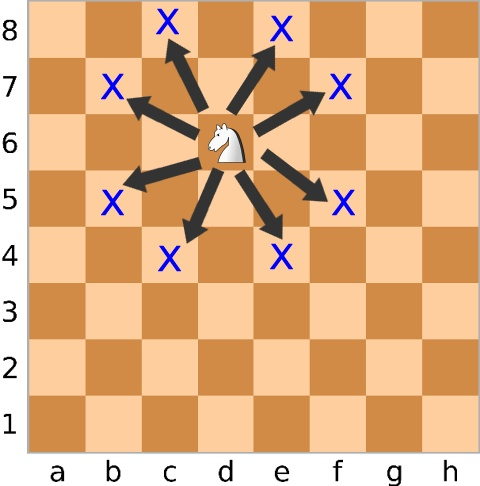
\includegraphics[width=0.37\linewidth]{deplacement-cavalier}
	\end{center}
	\caption{Illustration du mouvement d'un cavalier sur un échiquier}
\end{figure}

Dans un premier temps, les cases de l'échiquier sont représentées par des tuples~: le couple \texttt{(i,j)} désigne la case d'abscisse \texttt{i} et d'ordonnée \texttt{j}. Un échiquier possède 8 colonnes et 8 lignes, donc \texttt{i} et \texttt{j} seront compris entre \texttt{0} et \texttt{7}.

\question{\'Ecrire une fonction \texttt{estDansEch(i:int, j:int)->bool} qui renvoie \texttt{True} si \texttt{(i, j)} correspond à une case valide de l'échiquier et \texttt{False} sinon. }

\question{\'Ecrire une fonction \texttt{mvtsPossibles(i:int, j:int)->list} qui renvoie la liste des cases où le cavalier peut se déplacer à partir de la case \texttt{(i,j)} à l'ordre près.}

%\newpage
\question{Vérifier que :}
\vspace{-.2cm}
\begin{itemize}
	\item \texttt{mvtsPossibles(0,0)} renvoie \texttt{[(1, 2), (2, 1)]},
	\item \texttt{mvtsPossibles(3,5)} renvoie bien \texttt{[(1, 4), (1, 6), (2, 3), (2, 7), (4, 3), (4, 7), (5, 4), (5, 6)]},
	\item \texttt{mvtsPossibles(7,7)} renvoie bien \texttt{[(5, 6), (6, 5)]}.
\end{itemize}

Tous ces résultats sont à l'ordre près. 

\question{Créer un graphe \texttt{G} sous la forme d'un dictionnaire d'adjacence avec pour sommets les différentes cases de l'échiquier et les arêtes qui correspondent à un mouvement possible du cavalier. }

\question{Vérifiez que vous avez un graphe avec 64 sommets et 168 arêtes.}

Le codage des cases d'échiquier se fait classiquement par une chaine de caractères comprenant~: une lettre minuscule pour l'abscisse (de \texttt{a} à \texttt{h}) et un chiffre pour l'ordonnée (de \texttt{1} à \texttt{8}). La case en bas à gauche de l'échiquier est donc de code \texttt{'a1'}.

\begin{rem}
	\texttt{ord(c)} retourne le codage Unicode correspondant au caractère \texttt{c} et \texttt{chr(n)} renvoie le caractère dont le codage Unicode est \texttt{n}. 
\end{rem} 

\question{\'Ecrire une fonction \texttt{codage(i:int, j:int)->str} qui renvoie le code correspondant à la case \texttt{(i, j)}. }


\question{Créer un dictionnaire d'adjacence \texttt{G2} comme défini précédemment avec les cases maintenant nommées d'après leur code. }


\begin{figure}[h]
	\begin{center}
		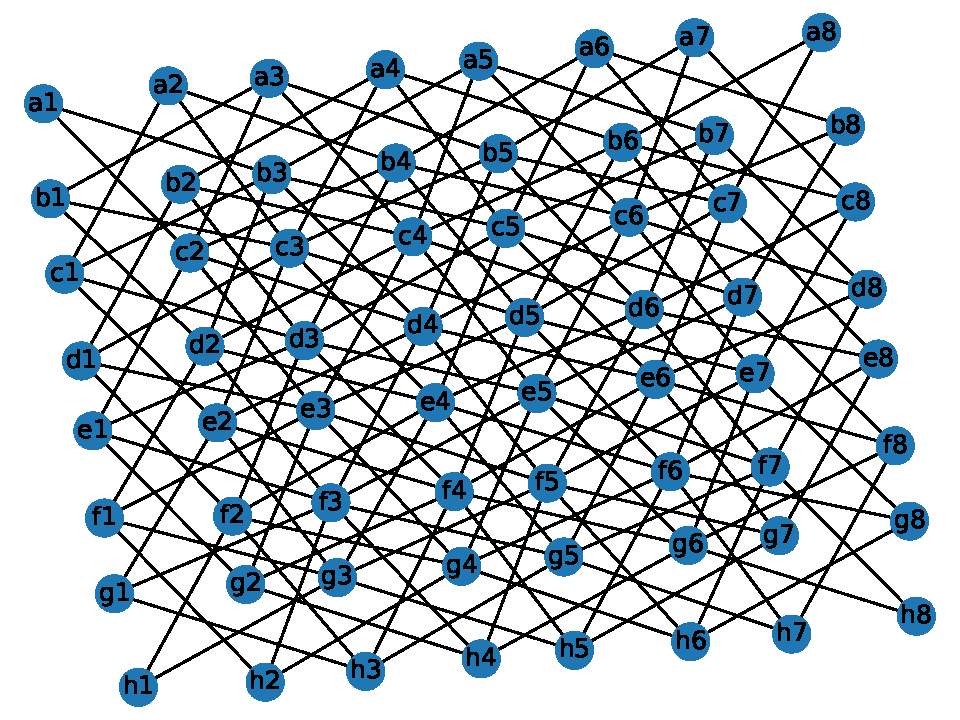
\includegraphics[width=0.7\linewidth]{Graphe_final}
	\end{center}
	\caption{Représentation graphique du graphe \texttt{G2}}
\end{figure}

\question{ Vérifier que~:
\begin{itemize}
	\item \texttt{G2['a1']} renvoie \texttt{['b3', 'c2']},
	\item \texttt{G2['d6']} renvoie bien \texttt{['b5', 'b7', 'c4', 'c8', 'e4', 'e8', 'f5', 'f7']},
	\item \texttt{G2['h8']} renvoie bien \texttt{['f7', 'g6']}.
\end{itemize}
Tous ces résultats sont à l'ordre près. }

\question{Écrire une fonction \cde{largeur\_dist(G:dict, dep:tuple)->dict:} qui prend en entrée un graphe
codé par un dictionnaire d’adjacence \cde{G} et un sommet de départ dep et renvoie un dictionnaire de distance à
partir du sommet \cde{dep}. Pour ce faire, vous vous inspirerez du parcours en largeur fourni. Si un sommet n’est
pas atteignable depuis le depuis \cde{dep}, la valeur associée doit être de \cde{-1}.}

\begin{lstlisting}
def bfs(G:dict, s) -> None:
    """
    G : graphe sous forme de dictionnaire d'adjacence
    s : sommet du graphe objet non mutable quelconque.
    """
    visited = {}
    for sommet,voisins in G.items():
        visited[sommet] = False
    # Le premier sommet à visiter entre dans la file
    file = deque([s])
    while len(file) > 0:
        # On visite la tête de file
        tete = file.pop()
        # On vérifier qu'elle n'a pas été visitée
        if not visited[tete]:
            # Si on ne l'avait pas visité, maintenant c'est le cas :)
            visited[tete] = True            
            # On met les voisins de tete dans la file
            for v in G[tete]:
                file.appendleft(v)
\end{lstlisting}

\question{Vérifier que vous obtenez le même résultat que sur la figure suivante en affichant les différentes valeurs de
distance depuis \cde{dep = (0, 0)} et \cde{dep = (4, 3)}. La fonction print peut ne pas revenir à la ligne si on précise un argument optionnel end différent de \cde{\\n}.}


\begin{figure}[H]
	\begin{center}
		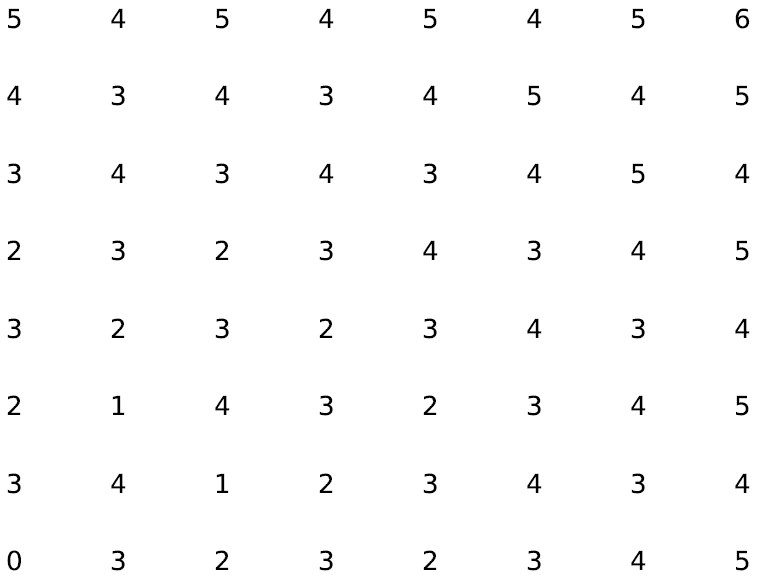
\includegraphics[width=0.45\linewidth]{distance_0_0}
\hfill
		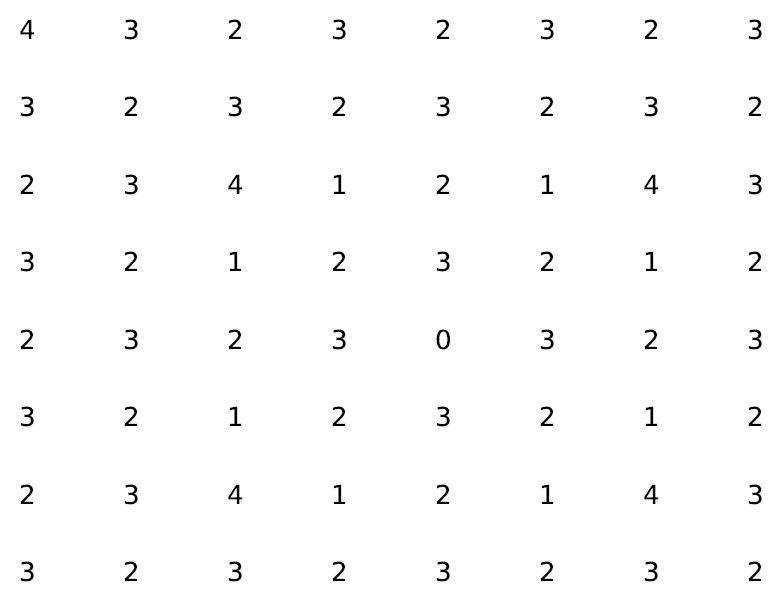
\includegraphics[width=0.45\linewidth]{distance_4_3}
	\end{center}
	\caption{Distances depuis \texttt{(0, 0)} et \texttt{(4, 3)}}
\end{figure}


\question{Pourquoi le parcours en profondeur n’est pas adapté à la résolution de ce problème ?}
